\begin{frame}
  \frametitle{Introducción a NoSQL}
\begin{itemize}
% \item Sobre los \~{}2010s, se renueva la búsqueda de la escalabilidad, con
%   el abaratamiento del {\em hardware}
% \item Se {\bf diversifican los problemas}, la inclusión del {\bf análisis
%     de todos los datos disponibles por parte de las empresas}
% \begin{itemize}
% \item incluso de algunos que no se había pensado usar, p. ej. {\em
%     clickstreams\/}), {\bf publicidad a la carta}, etc.
% \end{itemize}
\item {\bf NoSQL} \ra{} {\em hashtag\/} llamativo que se
  eligió para una conferencia en~2009 (Johan Oskarsson de Last.fm)
\item Ahora se asocia a cientos de bases de datos diferentes,
  que se han clasificado en varios tipos (las veremos después),
  caracterizadas por {\bf no usar SQL} como modelo de datos
\item {\bf NoSQL} \ra{} {\bfseries\itshape Not Only SQL} (no sólo SQL)
% \item Big Data \ra{} hay una variedad de fuentes de datos ({\bf persistencia
%     polígota})
  \end{itemize}
\end{frame}

% \begin{frame}
%   \frametitle{NoSQL}
% \centering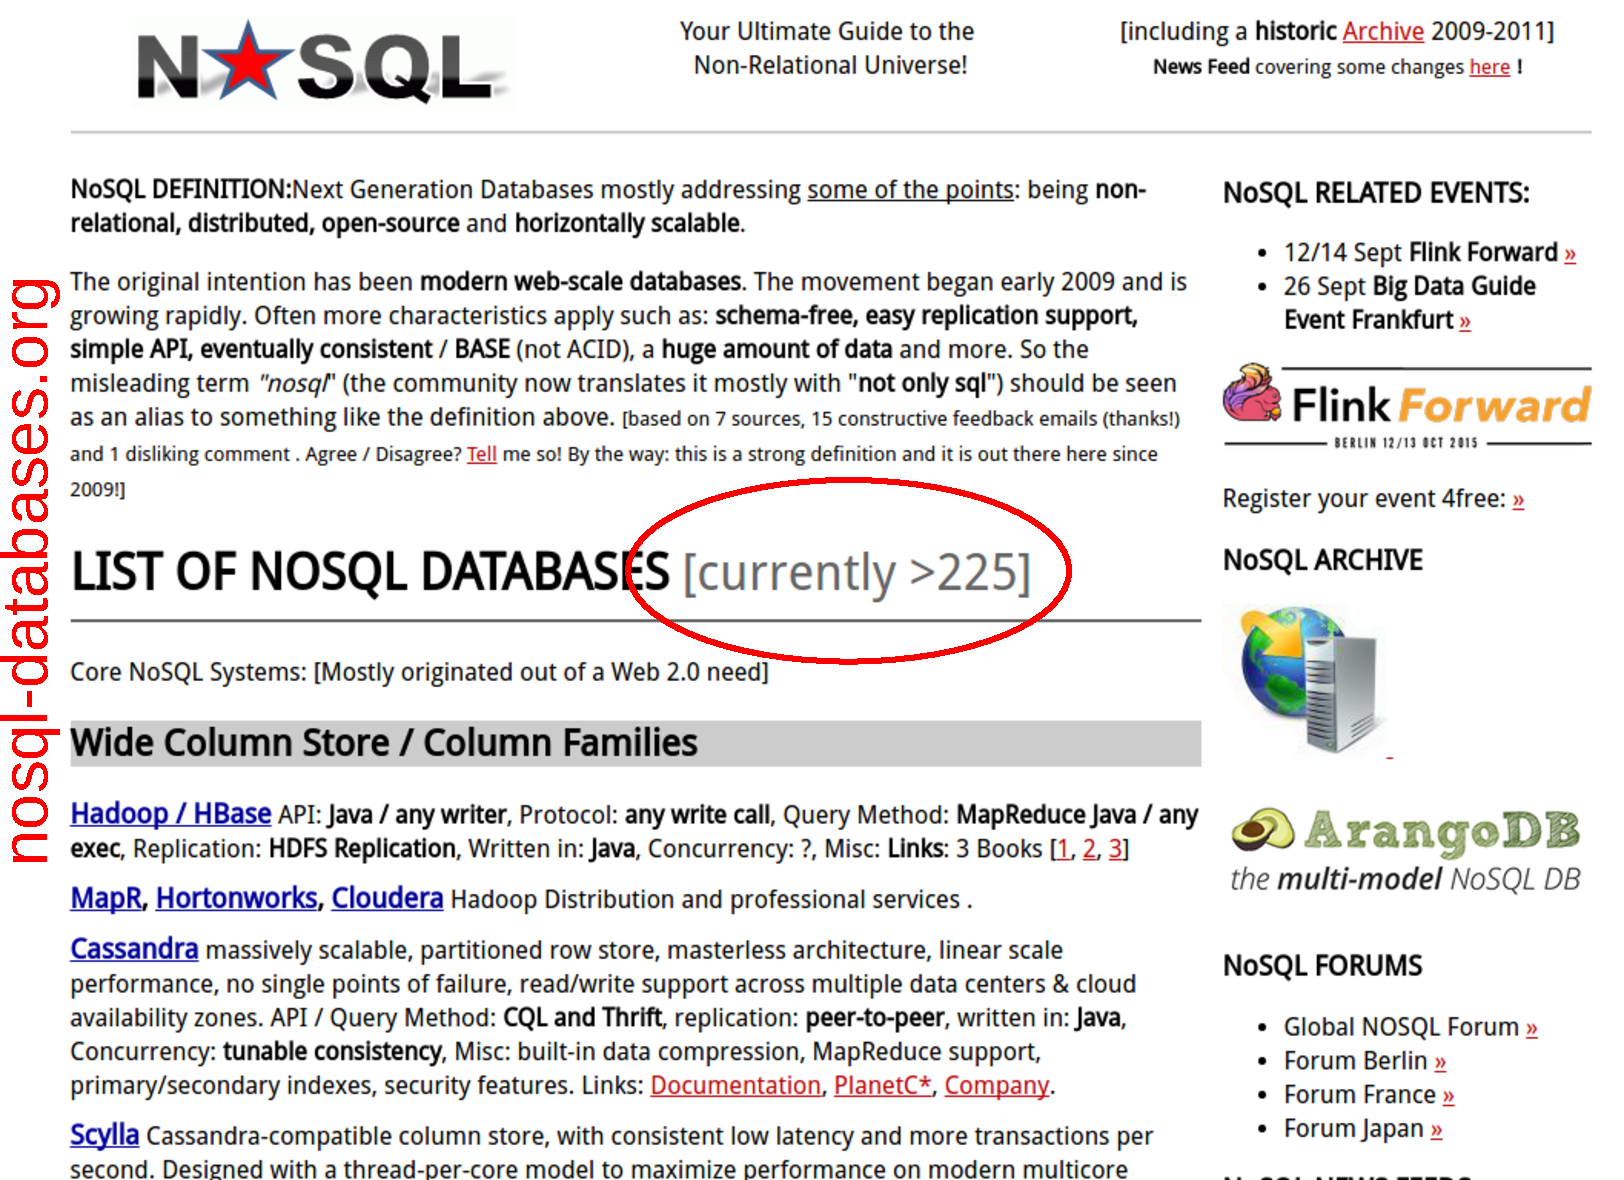
\includegraphics[width=\textwidth]{img/nosqldatabases3}
% \end{frame}

% \begin{frame}
%   \frametitle{NoSQL}
% \centering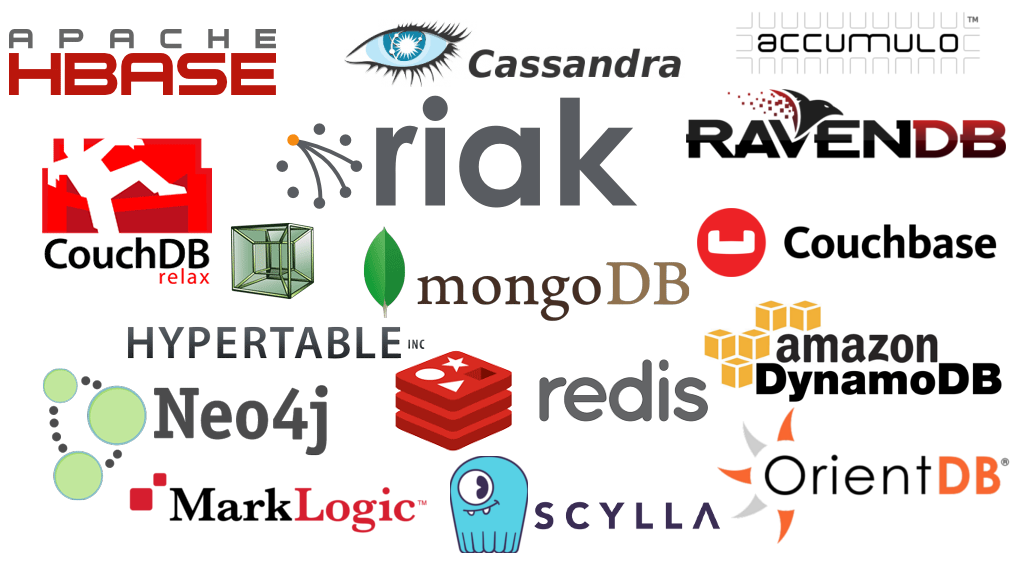
\includegraphics[width=\textwidth]{img/nosqldatabases}
% \end{frame}

\begin{frame}[allowframebreaks]
  \frametitle{NoSQL -- ¿Por qué se plantearon?}
%En general, el desarrollo de NoSQL ha venido motivado, entre otras, por una
%serie de circunstancias:
\begin{enumerate}
\item {\bf Mayor escalabilidad horizontal}
  \begin{itemize}
  \item conjuntos de datos muy muy grandes
  \item sistemas de alto volumen de escrituras ({\em streaming\/} de
    eventos, aplicaciones sociales)
  \end{itemize}
\item {\bf Demanda de productos de software libre} (crecimiento de las {\em
    start-ups})
\item {\bf Consultas especializadas} no eficientes en el modelo relacional
  (JOINs)
\item {\bf Expresividad, flexibilidad, dinamismo}. Frustración con {\bf
    restricciones} del modelo relacional
  % \ra{} ({\bfseries\itshape schemaless})
%\item Paradigma {\bf funcional}: {\em Map-Reduce}
\end{enumerate}

\framebreak

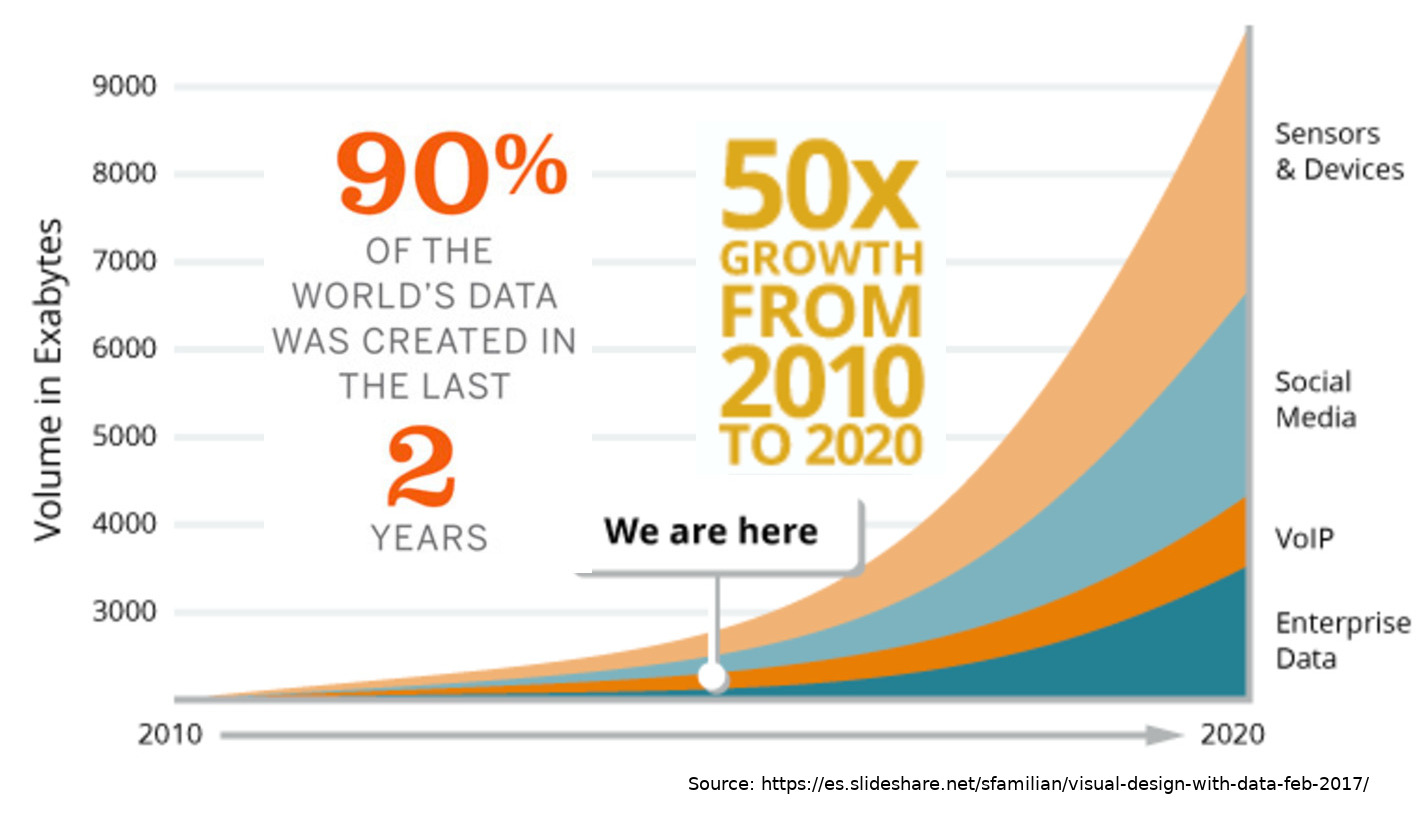
\includegraphics[width=\textwidth]{img/data-growth}

\end{frame}


\begin{frame}[allowframebreaks]
 \frametitle{NoSQL: Características}
\begin{itemize}
\item No se basan en SQL
\item Modelos de datos más ricos
\item Orientadas a la {\bf Escalabilidad}
\item Generalmente no obligan a definir un esquema \ra{}
  {\itshape\bfseries Schemaless}
\item Surgidos de la comunidad para solucionar problemas, y muchas de
  ellas son {\bf libres/{\itshape open source}}
\item Diseñadas \ra{} {\bf procesamiento distribuido}
\item Principios funcionales \ra{} {\bf MapReduce}
\item Generalmente implementan {\bf consistencia relajada}
\end{itemize}

% \framebreak

% \begin{block}{Categorías de NoSQL}
%     \begin{itemize}
%     \item Bases de datos Key-Value
%     \item Bases de datos Documentales
%     \item Bases de datos columnares
%     \item Bases de datos de grafos
%     \item Bases de datos de arrays
%     \end{itemize}
% \end{block}
\end{frame}


% \begin{frame}
%   \frametitle{Evolución desde el modelo relacional}
% \begin{itemize}
% \item El {\bf modelo relacional} $\Rightarrow$ {\bf predominante en los
%   últimos~\~{}30~años}
% \item Tiene sus raíces en el denominado {\em business data processing},
%   procesamiento de transacciones y {\em batch}
% \item Propuesto por Codd en los~70, {\bf de alto nivel}
% \item Actualmente los {\bf sistemas SQL están muy optimizados}:
% \begin{itemize}
% \item el {\bf grado de implantación es mayoritario}
% \item para el 99\% de los problemas (que caben en un ordenador) es
%   eficiente y adecuado
% \end{itemize}
% \end{itemize}
% \end{frame}

% % http://db-engines.com/en/ranking/


% \begin{frame}
%   \frametitle{Adopción de NoSQL}
% Twitter cambiando a Cassandra por~2010\\
% Cassandra desarrollada en Facebook en~2009\\
% 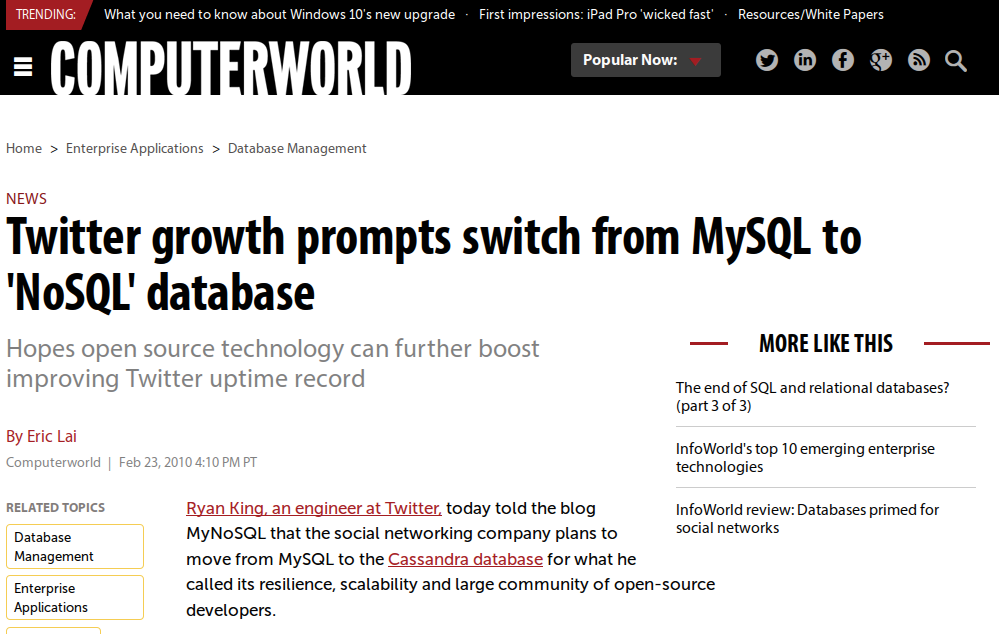
\includegraphics[width=\textwidth]{img/twitter-cassandra}
% \end{frame}

% \begin{frame}
%   \frametitle{Adopción NoSQL. Ranking julio 2017}
% \framesubtitle{Fuente: \url{http://db-engines.com/en/ranking/}}
% \vspace*{.1ex}
% \centering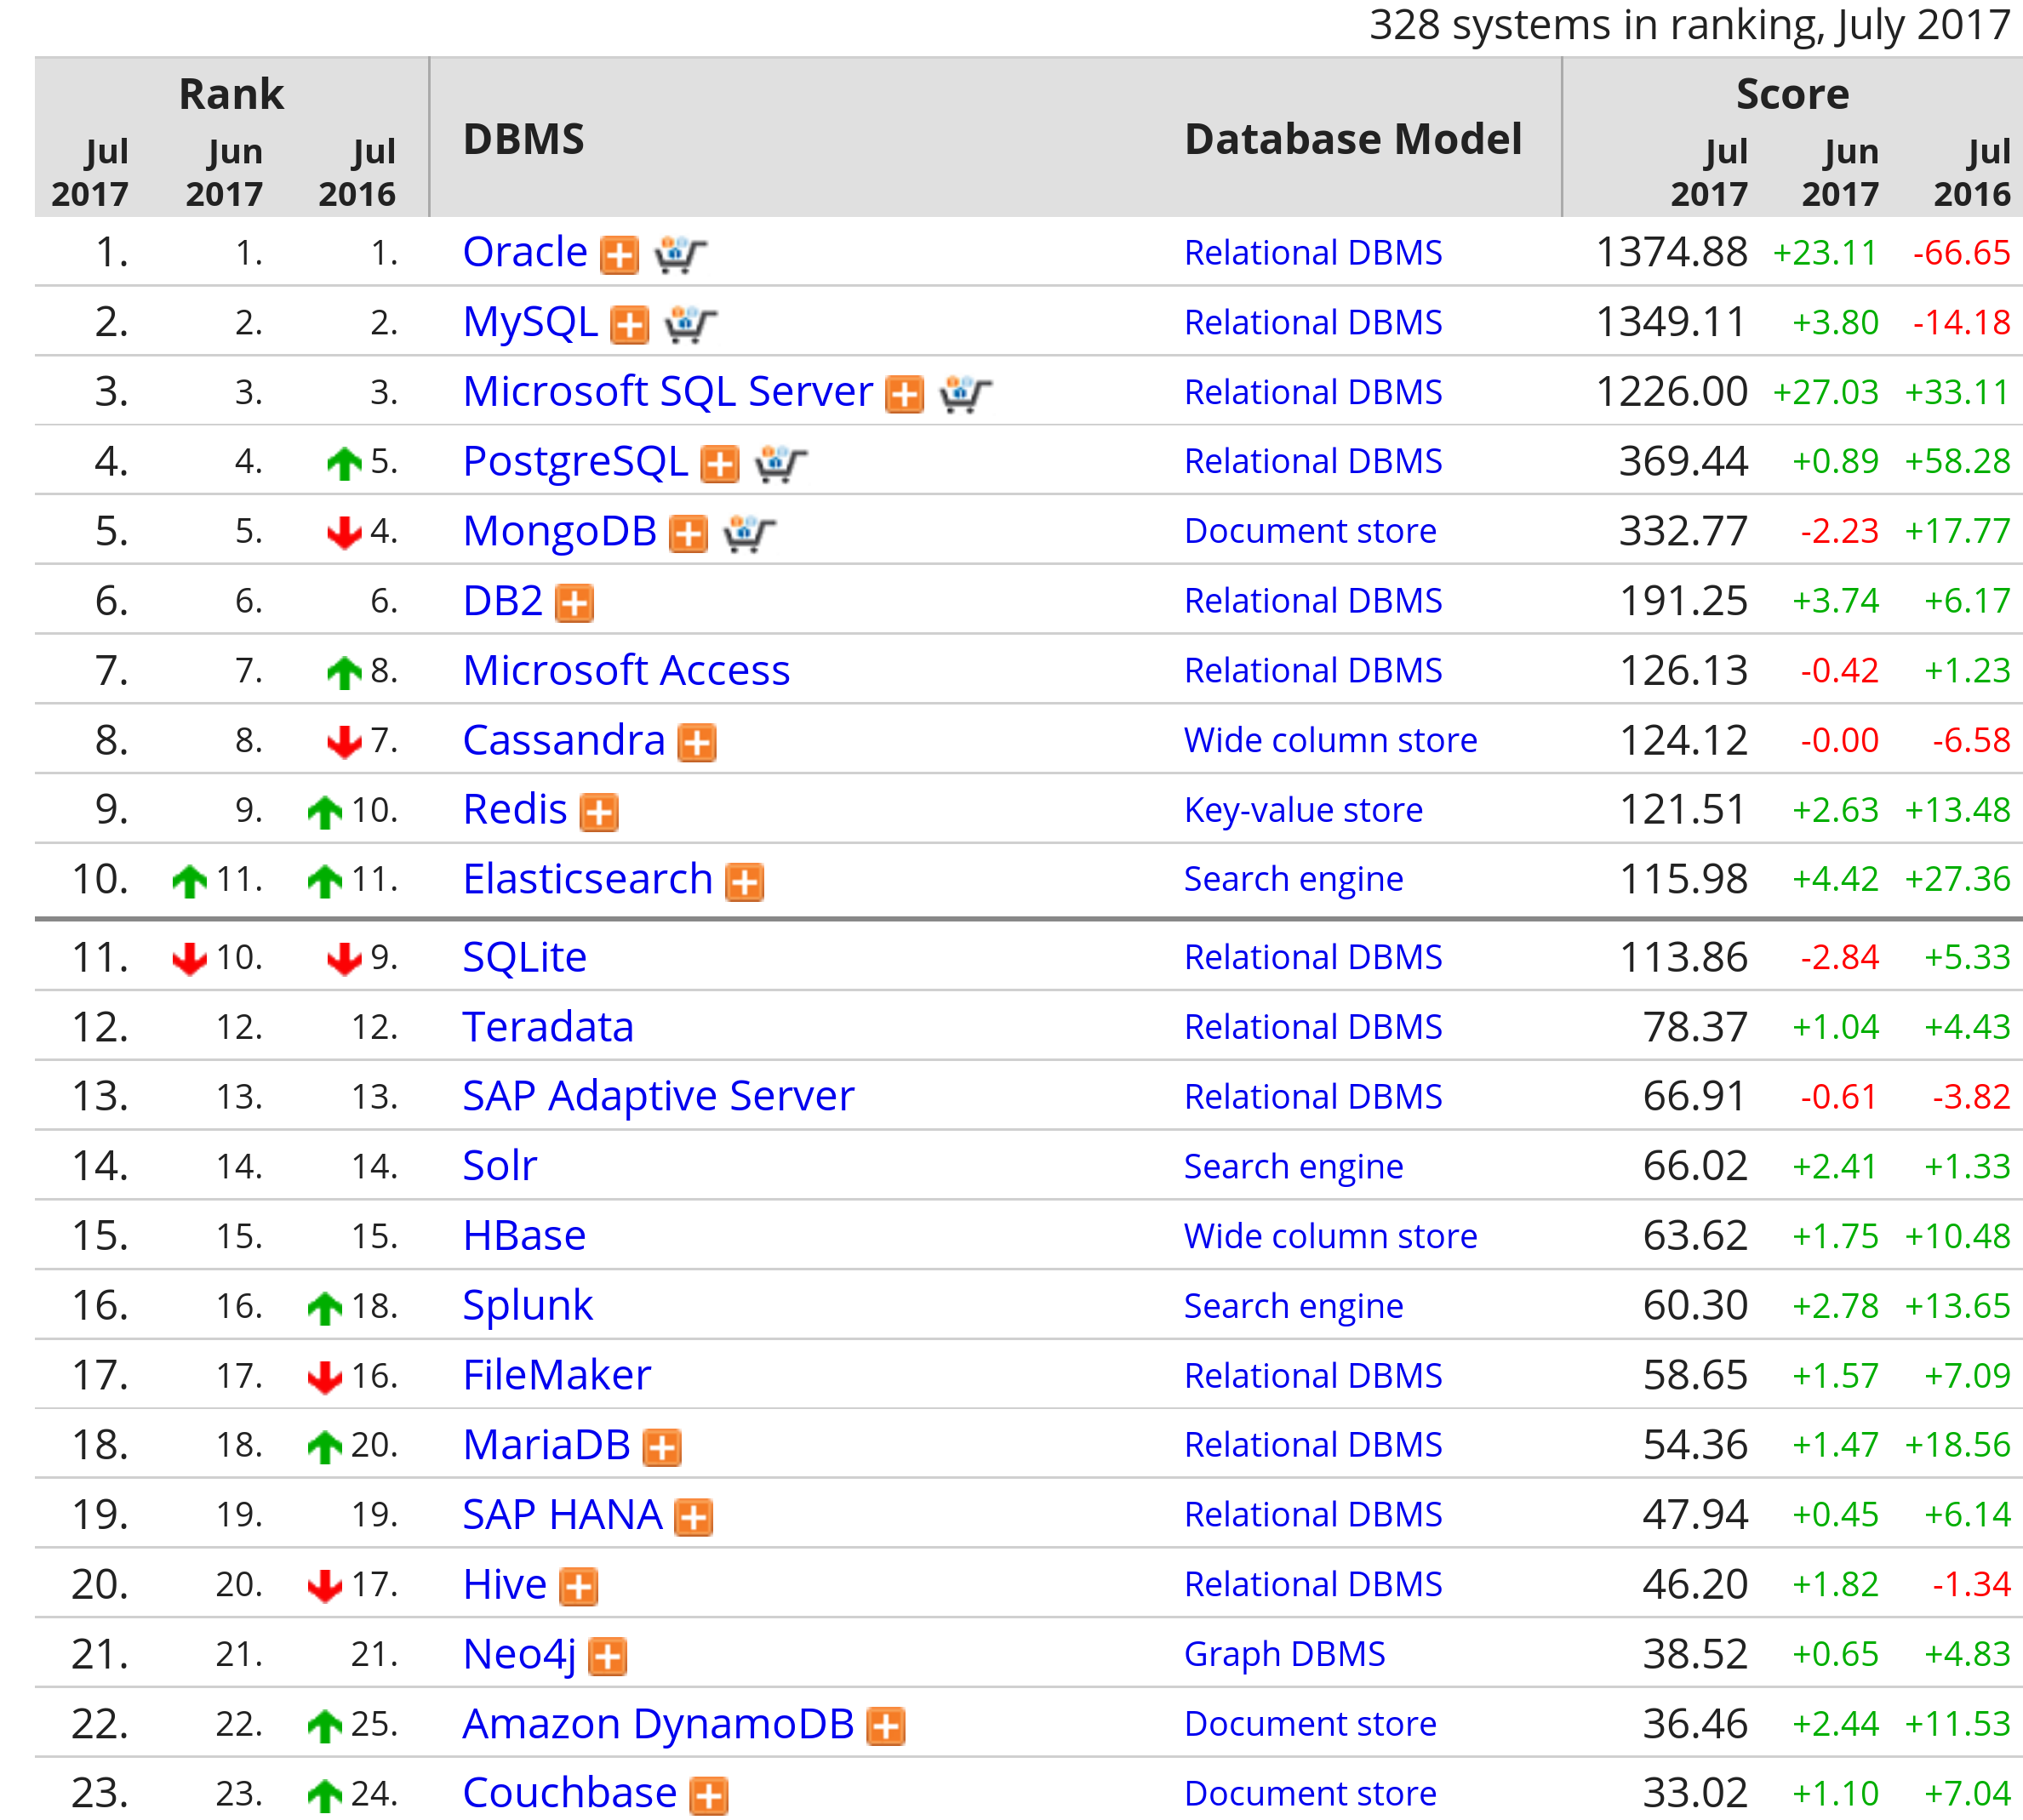
\includegraphics[width=.8\textwidth]{img/ranking-bbdd}
% \end{frame}

% \begin{frame}
% \frametitle{Adopción NoSQL.Tendencia julio 2017}
% \framesubtitle{Fuente: \url{http://db-engines.com/en/ranking/}}
% 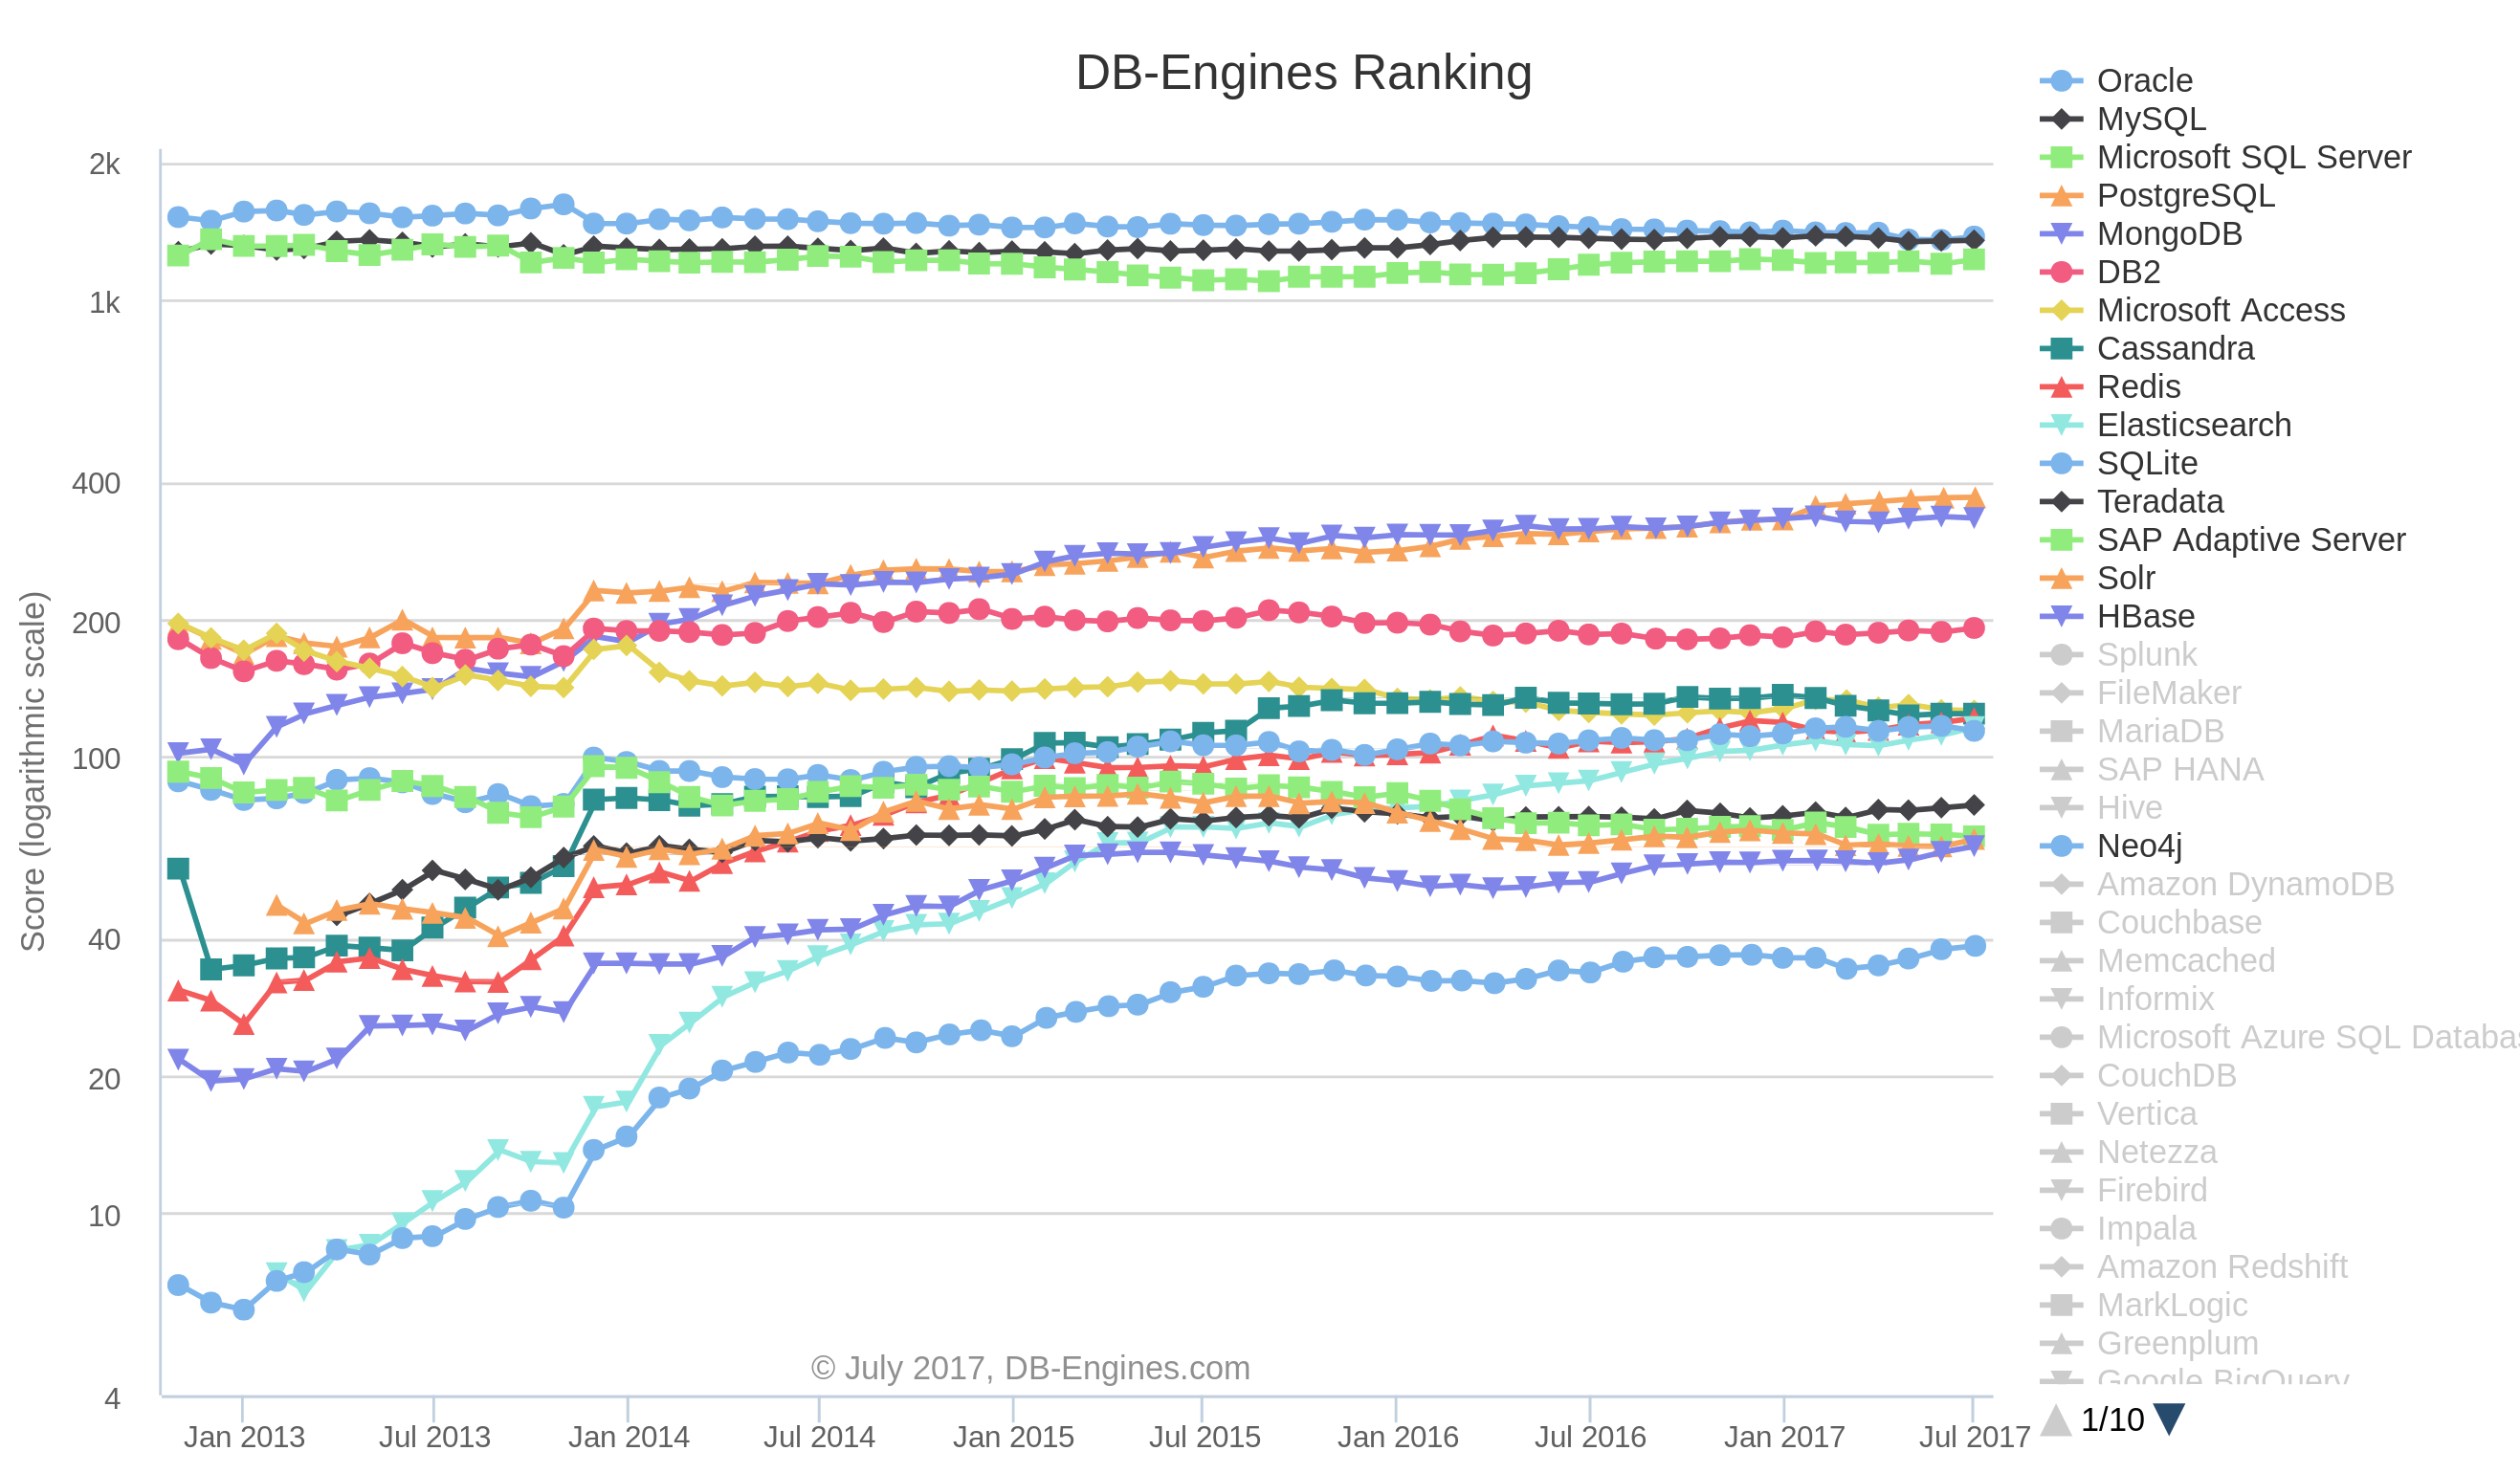
\includegraphics[width=\textwidth]{img/nosql-database-ranking}
% \end{frame}

% \begin{frame}
%   \frametitle{Adopción NoSQL. Análisis}
% \begin{alertblock}{Análisis}
% \begin{itemize}
% \item Dominan los grandes SGBDR
% \item El {\em Open Source} tiene una importancia crucial (MySQL,
%   MongoDB, etc.)
% \item Varias bases de datos NoSQL entre las~10 primeras. Muchas en las~20
%   primeras
% \item La distancia entre los grandes SGBDR y el primer NoSQL (MongoDB) es
%   de~5$\times$
% \item Paradigmas más ``atrevidos'' como el de grafos están entre los~20
%   primeros (Neo4j)
% \end{itemize}
%   \end{alertblock}
% \end{frame}



\subsection{La importancia de la escalabilidad}

\pgfdeclareimage[height=2.7em]{sobremesa}{img/server1}%img/servidor}
\pgfdeclareimage[height=.7em]{switch}{img/switch1}%img/switch}

\newsavebox{\network}

\begin{lrbox}{\network}
\begin{tikzpicture}
  \foreach \x in {0,...,5}
    \foreach \y in {0,...,3}
    \node [] (\x\y) at (1.5*\x,1.5*\y) {\pgfuseimage{sobremesa}};

% switch
\node[inner sep=0pt] (switch) at (1.5*2.5, 1.5*4) {\pgfuseimage{switch}};

\begin{scope}[on background layer]
  \foreach \x in {0,...,5}
    \foreach \y in {0,...,3}
      \draw[gray!50] (switch)--(\x\y) ;
\end{scope}
\end{tikzpicture}
\end{lrbox}

\begin{frame}
\frametitle{Cambio de perspectiva: Red}

\begin{overlayarea}{\textwidth}{.8\textheight}
\only<1->{%
\begin{center}
\usebox{\network}
\end{center}%
}%
% \only<2>{
% \vspace*{-13em}
%   \begin{block}{Almacenamiento distribuido}
%     \begin{itemize}
%     \item Desde los 90's: Clústers/NOC/COW: procesamiento masivamente
%       paralelo
% \begin{center}
% {\color{red}SIN EMBARGO...}
% \end{center}
% \item Almacenamiento no distribuido
% \item Ahora los nodos $\Rightarrow$ también {\bf almacenamiento}
% \item Minimizar el verdadero cuello de botella: {\bf trasiego de
%     información por la red}
%     \end{itemize}

%   \end{block}%
% }%
\only<2>{
\vspace*{-10em}
\begin{block}{Procesamiento distribuido}
\begin{itemize}
\item Necesidad de {\bf paralelización máxima}
\item {\bf Escalabilidad}
\item Explotación de la {\bf localidad de los datos}:
  \begin{itemize}
  \item Datos producidos en cada nodo se utilizan en siguientes iteraciones
  \item Cada nodo puede hacer de servidor para recibir datos
\end{itemize}
\end{itemize}
\end{block}
}%
\only<3>{
\vspace*{-9em}
\begin{block}{Procesamiento distribuido}
\begin{itemize}
\item Vuelta al modelo funcional inherentemente paralelo: (e.g. {\bf
    Map-Reduce})
\item Almacenamiento distribuido: (e.g. {\bf HDFS})
\item Coordinación distribuida: (e.g. {\bf Zookeeper})
\end{itemize}
\end{block}%
}%
% \only<4>{
% \vspace*{-13em}
% \begin{block}{Modelo de datos}
% \begin{itemize}
%   \item El modelo relacional limita a tablas con valores primitivos y
%     relaciones {\em Primary Key\/}/{\em Foreign Key}
%   \item Pero en programación se utilizan {\bf listas}, {\bf arrays}, {\bf
%       tipos de datos compuestos} ({\color{red}{\em gap\/} semántico})
%   \item ACID es {\bf muy compleja y costosa} en ambientes distribuidos
%     (quizá {\bf no necesaria} en algunas aplicaciones)
% \end{itemize}
% \end{block}%
% }%
\only<4>{
\vspace*{-10em}
\begin{block}{Modelo de datos}
\begin{itemize}
\item ¿Si se pudiera ver como un {\bf GRAN ARRAY}?
\begin{itemize}
\item Cada nodo almacenaría una parte del array
\item Búsqueda aleatoria {\bf muy rápida} (árboles B)
%\item Uso de {\bf filtros de Bloom}
\item Uso de {\bf objetos complejos} (p. ej. {\bf documentos JSON}),
  para mantener la {\bf localidad espacial de datos relacionados} (+
  después)
\item Transacciones limitadas al {\bf objeto complejo}
\end{itemize}
\end{itemize}
\end{block}%
}%
\end{overlayarea}
\end{frame}

\subsection{Schemaless}

\begin{frame}[fragile,allowframebreaks]
  \frametitle{Schemaless}
\begin{itemize}
\item Las BBDD NoSQL (en general) {\bf no requieren de un esquema}
\begin{alertblock}{}
  \centering
  \href{https://farm6.staticflickr.com/5483/29931060254_109e3e36da_o_d.jpg}{\bf
    SCHEMALESS}
\end{alertblock}
\item {\bf Flexibilidad}: Posibilidad de almacenar documentos con una
  estructura diferente
\begin{itemize}
\item Tratar información incompleta
\item Evolucionar la base de datos/esquema
\item Añadir nuevas características a las aplicaciones
\end{itemize}
\end{itemize}

\framebreak

\begin{small}
\begin{tabular}{p{.43\textwidth}cp{.43\textwidth}}
{\bfseries\itshape schema-on-write}&$\Rightarrow$&{\bfseries\itshape
                                                   schema-on-read}\\
\midrule
\rowcolor{blue!20} SQL&&NoSQL\\
\rowcolor{blue!15} Los datos conforman cuando se {\bf escriben}&&Los datos leídos conforman a
                                               un {\bf esquema implícito}\\
\rowcolor{blue!20} {\bf Tipado estricto} (estático) && {\bfseries\itshape Duck-Typing}
                                    (dinámico) \\
\rowcolor{blue!15}  Datos {\bf homogéneos} && Datos {\bf heterogéneos}\\
\rowcolor{blue!20} Proceso analítico a través de {\bf consultas} && {\bfseries\itshape Use as read}\\
\end{tabular}
\end{small}
% \item Se pasa de {\em schema-on-write} (se asegura que los
%   datos son conformes cuando se escriben, como en relacional) a {\em
%     schema-on-read} (los datos tienen un {\bfseries\itshape esquema
%     implícito} cuando se leen)
% \item Así, las bases de datos NoSQL están más cerca de los lenguajes
%   dinámicos, mientras que las relacionales más cerca de los lenguajes
%   estáticos
% \end{itemize}

\framebreak

\begin{itemize}
\item {\bf Ejemplo}: Añadir el campo {\tt first\_name} a partir del campo
  {\tt name}
\item Los nuevos objetos se crean con el nuevo formato
\item A la hora de leerlos, se puede hacer:
\end{itemize}
\begin{lstlisting}
if (user && user.name && !user.first_name) {
   // Docs anteriores a 2013 no tienen first_name
   user.first_name = user.name.split(" ")[0];
}
\end{lstlisting}

\framebreak

\begin{itemize}
\item En SQL:
  \begin{itemize}
  \item Puede ser un proceso muy costoso
  \item Procesa toda la tabla
  \item {\em Locking}
  \item Puede obligar a parar las aplicaciones
  \end{itemize}
\end{itemize}
\begin{lstlisting}[language=SQL]
ALTER TABLE users ADD COLUMN first_name text;
UPDATE users SET first_name =
    substring_index(name, ' ', 1);
\end{lstlisting}

\framebreak

\begin{block}{¿Cuándo es apropiado {\em schemaless}?}
  \begin{itemize}
  \item {\bf Objetos heterogéneos}
\item Estructura de los datos {\bf impuesta externamente}
\item Si intuimos que los datos {\bf cambiarán en el futuro}
  \end{itemize}
\end{block}


% \framebreak

% \begin{block}{SIN EMBARGO...}
%  A veces {\bf un esquema es conveniente}
% \begin{itemize}
% \item Facilita el desarrollo y evita inconsistencias
%   \begin{itemize}
%   \item {\tt Mongoose} para MongoDB:
%   \end{itemize}
% \end{itemize}
% \begin{lstlisting}[language=Java]
% var Comment = new Schema({
%   name: { type: String, default: 'Anonymous' },
%   date: { type: Date, default: Date.now },
%   text: Buffer
% });
% // a setter with on-line modification
% Comment.path('name').set(function (v) {
%   return capitalize(v);
% });
% \end{lstlisting}
% \end{block}
\end{frame}


% \begin{frame}
%   \frametitle{Choose wisely}
% \begin{columns}
% \begin{column}{.5\textwidth}
%   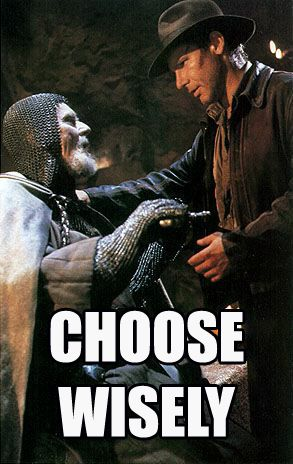
\includegraphics[height=.7\textheight]{img/chose-wisely}
% \end{column}
% \begin{column}{.5\textwidth}
% \begin{alertblock}{SQL}
% \end{alertblock}
% \begin{alertblock}{NoSQL}
% \end{alertblock}
% \begin{alertblock}{Polyglot Persistence}
% \end{alertblock}
% \end{column}
% \end{columns}
% \end{frame}


\subsection{Modelado de datos en NoSQL}

\begin{frame}[allowframebreaks]
  \frametitle{Modelado de datos en NoSQL}

\begin{itemize}
\item En general ofrecen más {\bf flexibilidad} en el modelado de datos:
  \begin{itemize}
  \item {\bf Documentos}: Posibilidad de {\bf agregación} (además de
    referencia)
  \item {\bf Grafos}: Gran número de relaciones entre elementos
  \end{itemize}
\item {\bf Optimización guiada por las consultas}
\item Es ``barato'' {\bf duplicar (desnormalizar)} los datos si con ello se
  consigue {\bf mayor eficiencia de acceso}
\end{itemize}

%   \framebreak
% Con respecto al modelo de datos:

% \begin{itemize}
% \item Se mantienen los conceptos de entidad, relación, cardinalidades, etc.
% \item El modelado relacional se centra en especificar {\bf qué datos
%     tenemos y podemos ofrecer}
% \item El modelo NoSQL se centra en {\bf optimizar qué
%     consultas vamos a servir}
% \end{itemize}

\end{frame}

\begin{frame}
  \frametitle{Representación relacional de un CV}
\framesubtitle{Kleppmann, 2016. \emph{Designing Data Intensive Applications}}
  \centering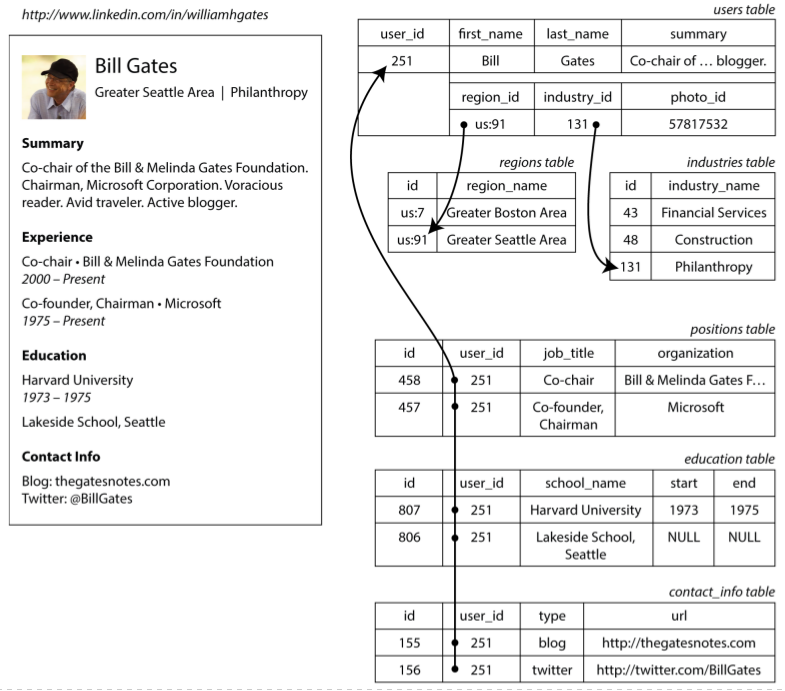
\includegraphics[height=.81\textheight]{img/gates}
\end{frame}

% \begin{frame}
%   \frametitle{Representación de relaciones}

%   Las relaciones uno a muchos (e.g. {\tt positions}) en el modelo
%   relacional:

% \begin{itemize}
% \item Normalización usando varias tablas ({\tt Positions} con
%   {\tt user\_id})
%   \begin{itemize}
%   \item Necesidad de más de una tabla
%   \item Necesidad de uso de {\tt JOIN} $\Rightarrow$ ineficiencia
%   \end{itemize}
% \item Algunos SGBDR ofrecen la posibilidad de tener tipos de datos
%   estructurados y campos XML o JSON. (P. ej. PostgreSQL)
%   \begin{itemize}
%   \item Alternativa interesante, aunque...
%   \item No son estándar
%   \end{itemize}
% \end{itemize}
% \end{frame}

\begin{frame}[plain,fragile]
%  \frametitle{CV como un documento}
\begin{lstlisting}[language=json,basicstyle=\tiny\tt]
{
  "user_id": 251,
  "first_name": "Bill",
  "last_name": "Gates",
  "summary": "Co-chair of the Bill & Melinda Gates... Active blogger.",
  "region_id": "us:91",
  "industry_id": 131,
  "photo_url": "/p/7/000/253/05b/308dd6e.jpg",
  "positions": [
    {
      "job_title": "Co-chair",
      "organization": "Bill & Melinda Gates Foundation"
    },
    {
      "job_title": "Co-founder, Chairman",
      "organization": "Microsoft"
    }
  ],
  "education": [
    {
      "school_name": "Harvard University",
      "start": 1973,
      "end": 1975
    },
    {
      "school_name": "Lakeside School, Seattle",
      "start": null,
      "end": null
    }
  ],
  "contact_info": {
    "blog": "http://thegatesnotes.com",
    "twitter": "http://twitter.com/BillGates"
  }
}
\end{lstlisting}
\end{frame}

% \begin{frame}
%   \frametitle{CV como un árbol (equivalente)}
% \centering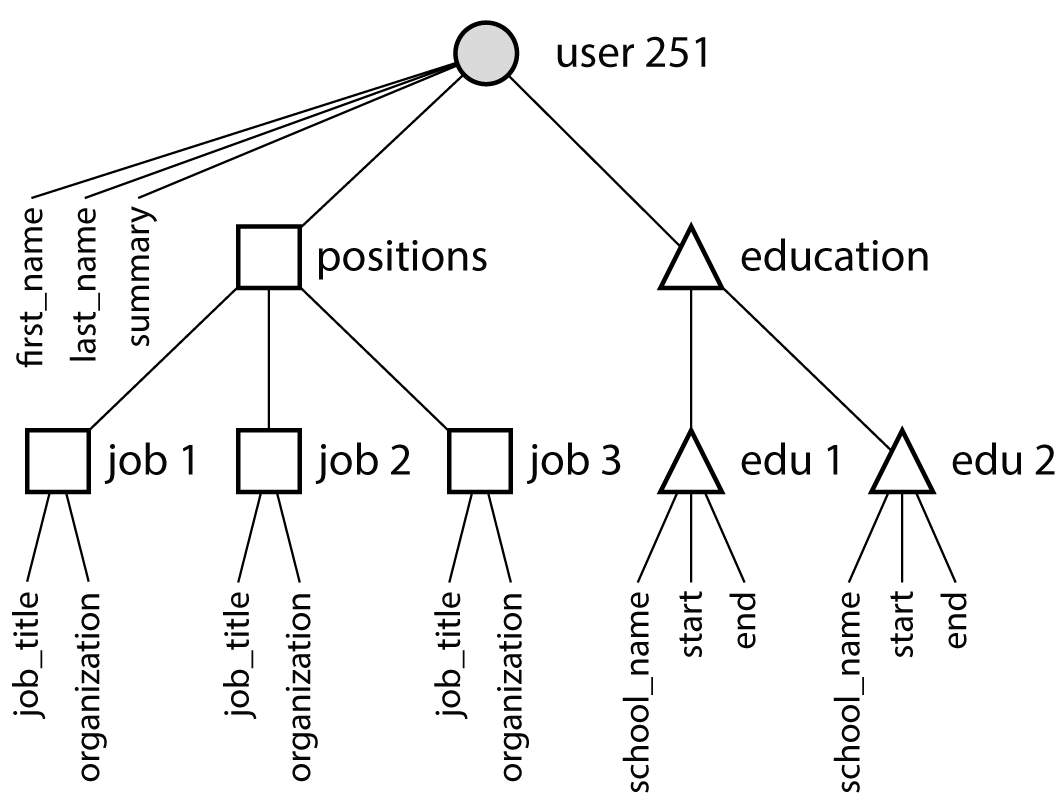
\includegraphics[height=.85\textheight]{img/tree}
% \end{frame}

% \begin{frame}[allowframebreaks]
%   \frametitle{Representación de Relaciones}
% \framesubtitle{Modelo de documentos}
% \begin{itemize}
% \item {\bf Modelo de documentos} \ra{} analogía del {\bf array/mapa
%     gigante}
% \item {\bf Conjunto de documentos} (objetos complejos)
%   \begin{itemize}
% \item Un {\bf identificador único}, campo {\em id\/}
% \item Búsqueda aleatoria eficiente por clave ({\bf referencia})
% \item Estructura jerárquica de sub-documentos contenidos \ra{}
%   {\bf agregación}
% \end{itemize}
% \end{itemize}


% \begin{alertblock}{}
%   Más flexibilidad que el modelo relacional (elección entre \underline{\em
%     referencia} y \underline{\em agregación})
% \end{alertblock}

% \end{frame}

% \begin{frame}[allowframebreaks]
%   \frametitle{Representación de Relaciones}
% \framesubtitle{Uno a muchos (ii) -- NoSQL}
% \begin{itemize}
% \item Relaciones {\bf Uno a Muchos} ({\tt positions}):
%   \begin{itemize}
%   \item {\bf Opción 1}: Agregando la tabla {\tt positions}
%   \item {\bf Opción 2}: Convertir las empresas en entidades, y utilizar una
%     {\bfseries\itshape referencia}
%   \end{itemize}
% \item ¿Qué opción elegir?
% \end{itemize}

% \framebreak

% \begin{alertblock}{¡Modelo guiado por el acceso a datos!}
% \begin{small}
%   \begin{itemize}
%   \item Si los elementos ``muchos'' tienen una estructura sencilla
%     \ra{} {\bf Opción~1}
% \item Si los elementos ``muchos'' son usualmente {\bf recuperados en una
%     consulta} junto con el elemento ``uno'' \ra{} {\bf Opción~1}
% \item Si los elementos ``muchos'' son relativamente grandes, o bien son
%   recuperados siempre de forma separada \ra{} {\bf Opción~2}
%   \end{itemize}
% \end{small}
% \end{alertblock}
% \end{frame}

% \begin{frame}
%   \frametitle{Representación de Relaciones}
%   \framesubtitle{Muchos a uno y muchos a muchos}
% Relaciones muchos a uno y muchos a muchos:
%     \begin{itemize}
%     \item Personas que viven en una región
% \item Preguntas que refieren a Tags
%     \end{itemize}
% El modelo de documentos no aporta ventajas
%   \begin{itemize}
%   \item La {\em agregación} daría lugar a mucha {\bf duplicación} (y a
%   problemas de sincronización)

% \item {\color{red} $\Rightarrow$} {\bf Referencias} (sobre el ID), similar
%   a una FK en el modelo relacional
% \begin{itemize}
%   \item {\color{red} $\Rightarrow$} al no haber {\bf JOINs} la aplicación
%     tiene que hacer más de una petición a la BD
%   \end{itemize}
% \end{itemize}
% \end{frame}

% \begin{frame}
%   \frametitle{Muchos a muchos -- referencia}
% 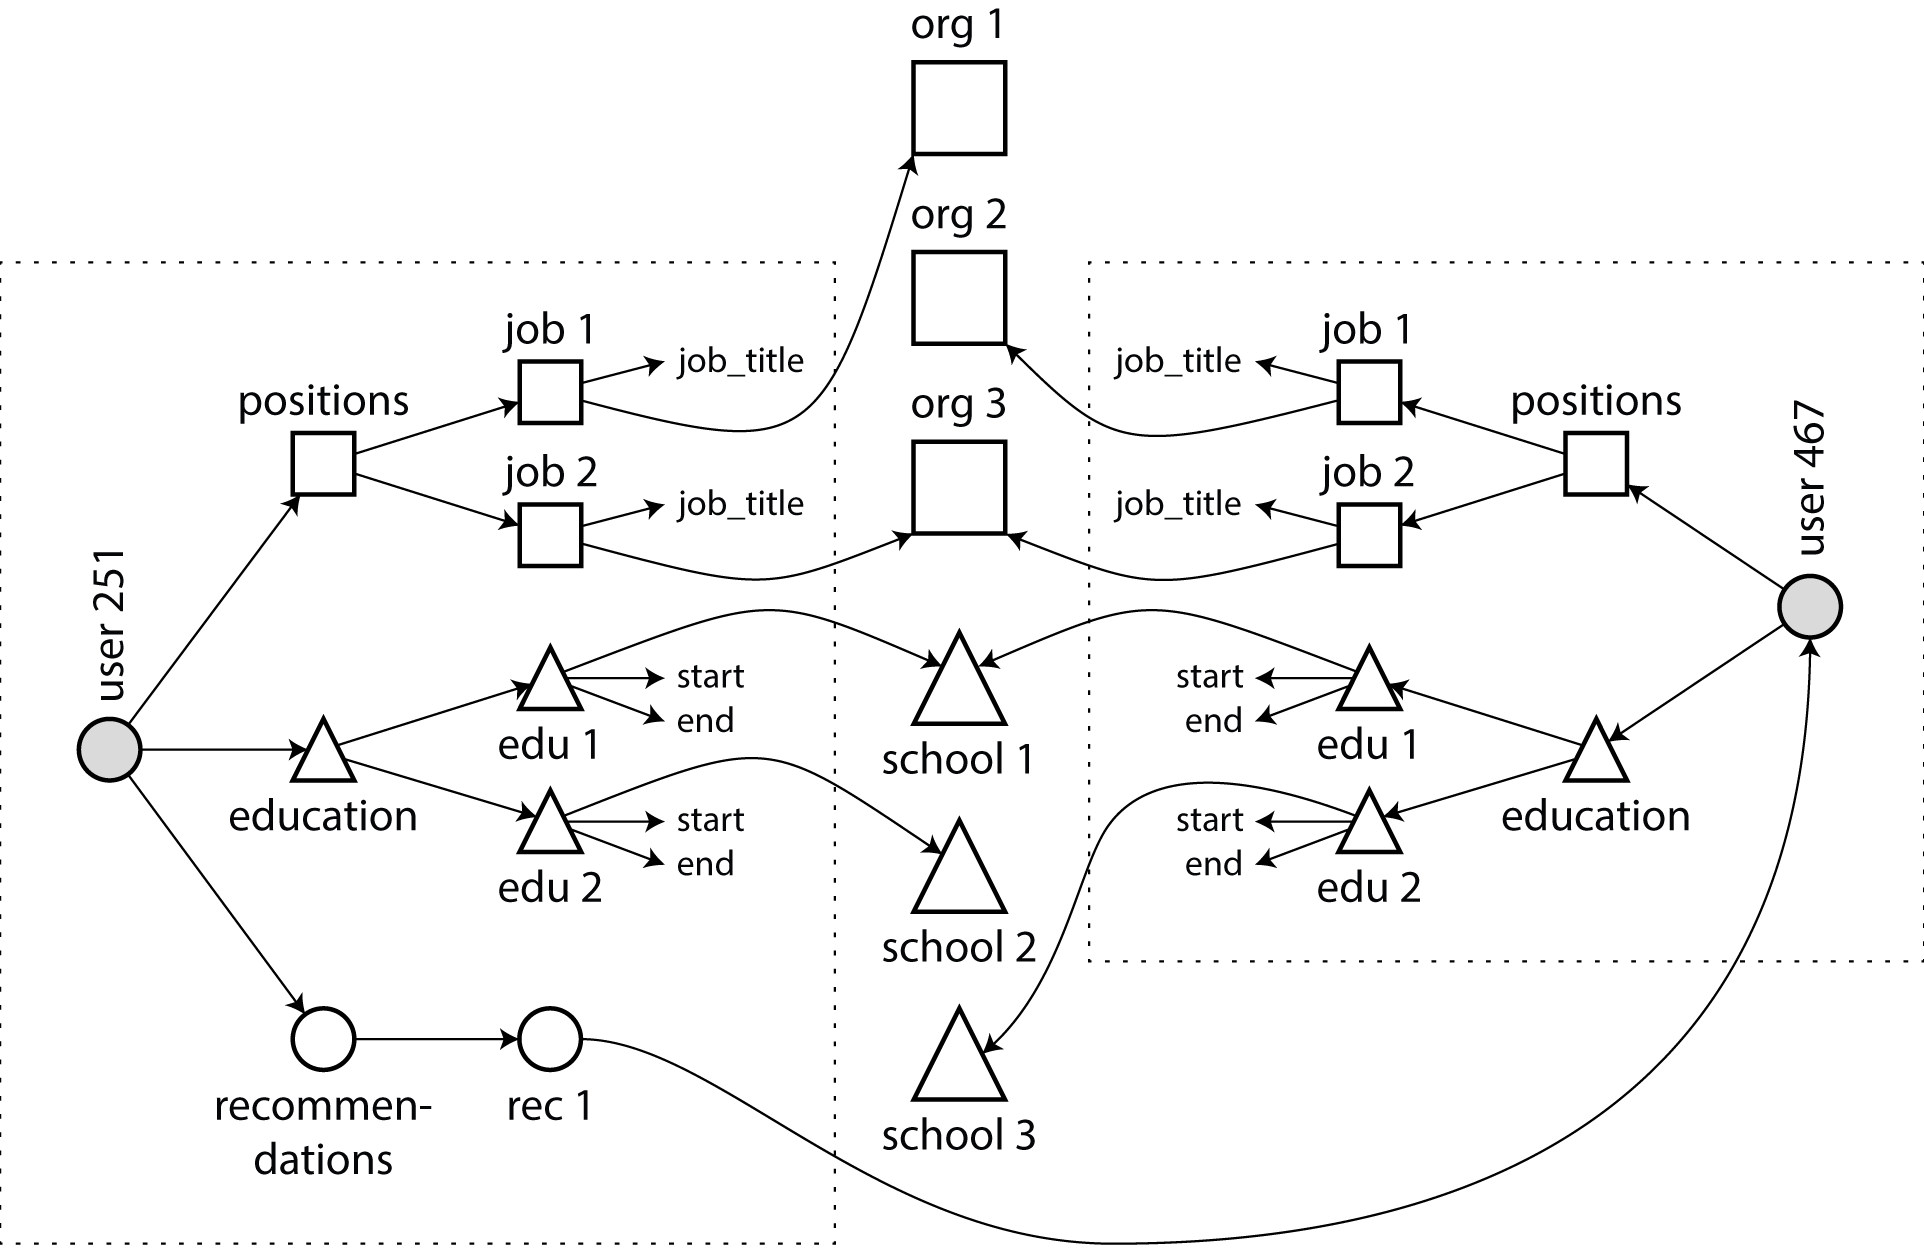
\includegraphics[width=\textwidth]{img/many-to-many}
% \end{frame}

% \begin{frame}
%   \frametitle{Reconsiderando el modelo de documentos}
%   \begin{itemize}
%   \item Las ventajas del modelo basado en documentos son:
%     \begin{itemize}
%     \item Para algunas aplicaciones, la abstracción de documentos se acerca
%       más al modelo de datos
% \item La abstracción de documentos aporta más flexibilidad al esquema. Por
%   ejemplo, se pueden añadir campos diferentes a cada documento (también
%   llamados modelos {\itshape\bfseries schemaless\/})
% \item En algunos casos puede mejorar la eficiencia gracias a la localidad
%   (agregación)
%     \end{itemize}
%   \end{itemize}
% \end{frame}


% \subsection{Eficiencia {\em raw}}

% \begin{frame}[allowframebreaks]
%   \frametitle{Eficiencia {\em raw}}
%   \begin{itemize}
%   \item Los sistemas NoSQL tienen que competir también con los SQL en
%     términos de eficiencia neta (también llamada {\em raw})
%   \item Un pequeño test sintético nos puede ayudar a hacernos una
%     idea\footnote{\url{http://bonesmoses.org/2016/07/15/pg-phriday-a-postgres-persepctive-on-mongodb/}.}

%   \item La prueba se realizó sobre MongoDB y sobre MySQL (se ha adaptado el
%     original, que era para PostgreSQL)\footnote{Datos disponibles en:
%       \url{https://github.com/dsevilla/bdge/tree/master/addendum}.}

%   \framebreak

% \item Se parte de una tabla sencilla con cuatro valores, que muestran
%   medidas de sensores con localización, valor de la lectura y una marca de
%   tiempo
%   \item Se realizan seis pruebas que pueden corresponder a un conjunto de
%     consultas normales:
%   \framebreak
%   \begin{enumerate}
%   \item Inicialmente se insertan {\bf un millón} de elementos generados al
%     azar, con fechas que permitan la búsqueda por rango ({\bf Fill})
%   \item Se crea un índice en la tabla para la fecha de la lectura ({\bf
%       Index})
%   \item Se actualizan los valores de un conjunto de entradas seleccionadas
%     por rango de fechas ({\bf Update})
%   \item Se eliminan un conjunto de filas seleccionadas por rango de fechas
%     ({\bf Delete})
%   \item Obtiene el número de filas restantes ({\bf Count})
%   \item Se obtiene un {\bf subconjunto} de filas extraído de una consulta
%     dada por un rango de fechas ({\bf Interval})
%   \end{enumerate}

% \end{itemize}

% \begin{center}
% 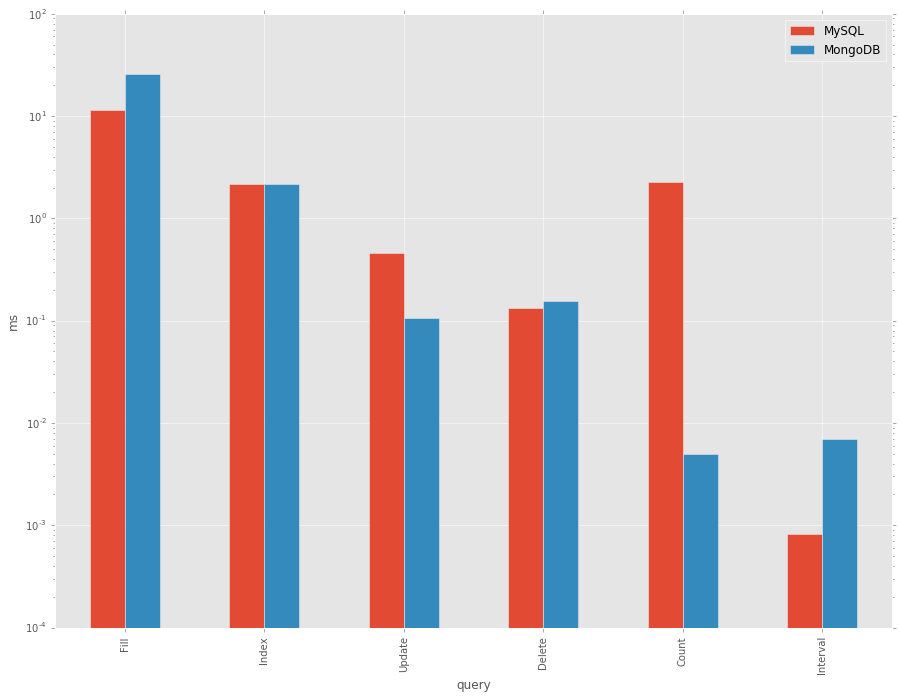
\includegraphics[width=.9\textwidth]{img/mongo_vs_mysql}
% \end{center}


% \begin{itemize}
% \item El gráfico tiene escala logarítmica en el eje Y (las
%   diferencias pequeñas se acentúan)
% \item A simple vista, ambos están muy igualados
%   \begin{itemize}
%   \item SQL (MySQL) lleva {\em muchos años} de optimizaciones
%   \item MongoDB tiene menos historia a sus espaldas en cuanto a
%     optimizaciones, etc.
%   \end{itemize}
% \item Hay casos en los que uno es más rápido que el otro y viceversa

% \framebreak

% \item No se puede decir cuál es mejor
%   \begin{itemize}
%   \item {\bf \color{red} $\Rightarrow$ DEPENDE DEL PATRÓN DE ACCESOS QUE VAYA A
%       TENER NUESTRA APLICACIÓN}
%   \item (p. ej. contado en MongoDB mucho más rápido que en MySQL;
%     actualización algo más rápida)
%   \end{itemize}
% \end{itemize}

% \end{frame}

% \begin{frame}
%   \frametitle{Map-Reduce}
% \begin{itemize}
% \item La escalabilidad de las bases de datos relacionales está limitada por
%   la ley de Moore
% \item Los {\em clústers} surgieron como una alternativa para proporcionar
%   {\em escalabilidad horizontal} (vs. escalabilidad vertical, mejorar un
%   procesador)
% \item Sin embargo, las bases de datos relacionales no casan bien con los
%   clústers ({\em joins} en tablas muy grandes, tablas temporales, etc.)
% \item Como se ha dicho, las bases de datos NoSQL surgieron como una
%   respuesta a estas limitaciones
%   \begin{itemize}
%   \item Al preferir la {\bf agregación} (localidad) a la referencia (claves
%     ajenas), cada entidad almacenada se hace más independiente
% \item Por lo tanto, se puede almacenar de forma más sencilla en un {\em
%     pool} de servidores
% \item Se adoptó también el paradigma funcional de procesamiento de datos
%   $\Rightarrow$ {\bf Map-Reduce}
% \item Millones de máquinas ejecutan {\bf en paralelo procesos} sobre datos
%   que están {\bf físicamente distribuidos}, alojando los resultados {\bf
%     localmente en cada servidor} (descentralización, HDFS, Hadoop, etc.)
%   \end{itemize}
%   \end{itemize}
% \end{frame}

%%% Local variables:
%%% mode: LaTeX
%%% TeX-master: "slides.tex"
%%% ispell-local-dictionary: "spanish"
%%% fill-column: 75
%%% TeX-parse-self: t
%%% TeX-auto-save: t
%%% End:
%%% vim: expandtab shiftwidth=2 tabstop=2
